% template created by: Russell Haering. arr. Joseph Crop
\documentclass[12pt,letterpaper]{article}
\usepackage{anysize}
\usepackage{cite}
\usepackage{amsmath,amssymb,amsfonts}
\usepackage{algorithm}
\usepackage[noend]{algpseudocode}
\usepackage{graphicx}
\usepackage{multirow}
\usepackage{listings}
\usepackage{xcolor}


\marginsize{2cm}{2cm}{1cm}{1cm}

\lstset{ framexleftmargin=9mm, frame=shadowbox,tabsize = 4}

\begin{document}

\begin{titlepage}
    \vspace*{4cm}
    \begin{flushright}
    {\huge
        ECE 375 Lab 7\\[1cm]
    }
    {\large
    	Remotely communicated Rock Paper Scissors
    }
    \end{flushright}
    \begin{flushleft}
    Lab session: 015
    
    Time: 12:00-13:50
    \end{flushleft}
    \begin{flushright}
    Author: Astrid Delestine

    Programming partner: Lucas Plastid 

    \vfill
    \rule{5in}{.5mm}\\
    TA Signature
    \end{flushright}

\end{titlepage}

\section{Introduction}
%This is the first Lab in the ECE 375 series and it covers the setup and compilation of an AVR Assembly Program. The student will learn how how to use the sample Basic Bump Bot assembly file and send the binaries to the AVR Microcontroller board. For the second part of the lab the student will be expected to download and compile the included C sample program and from it learn how to configure the I/O ports of the ATmega32U4 Microcontroller. The student will then write their own C program and upload it to the Microcontroller to verify that it runs as expected. The provided programs have been attached in the source code section of this report.
This is the final lab for ECE 375 and as such it necessitates a challenge. The major task for this lab was to, with 2 Benny boards, have them communicate over USART to play a game of rock paper scissors with each other. This allowed the students to apply certain knowledge gained about timers/counters, and how they can apply when sending or receiving data.


\section{Design}
The design for this Lab can be seen below in the flow chart and the derision tree that we built.

\begin{figure}[h]
	\centering
	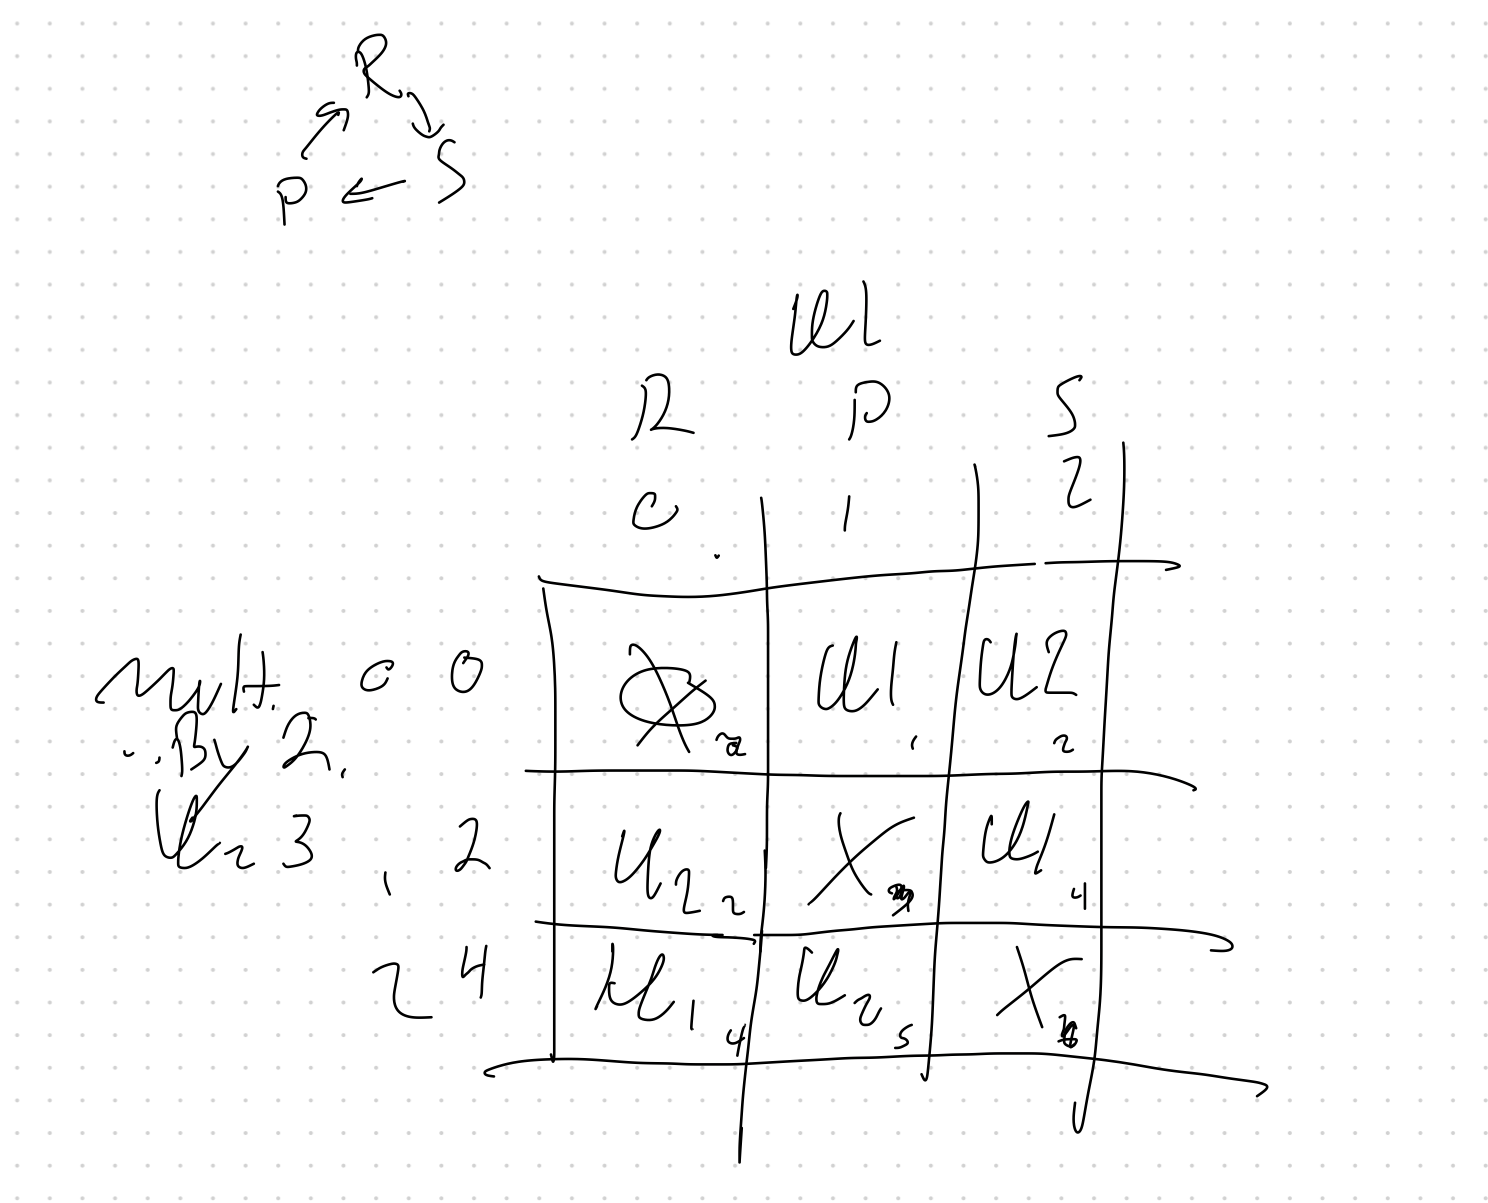
\includegraphics[width=12cm, height=10cm]{boxBreakdown.png}

\end{figure}

\begin{figure}[h]
	\centering
	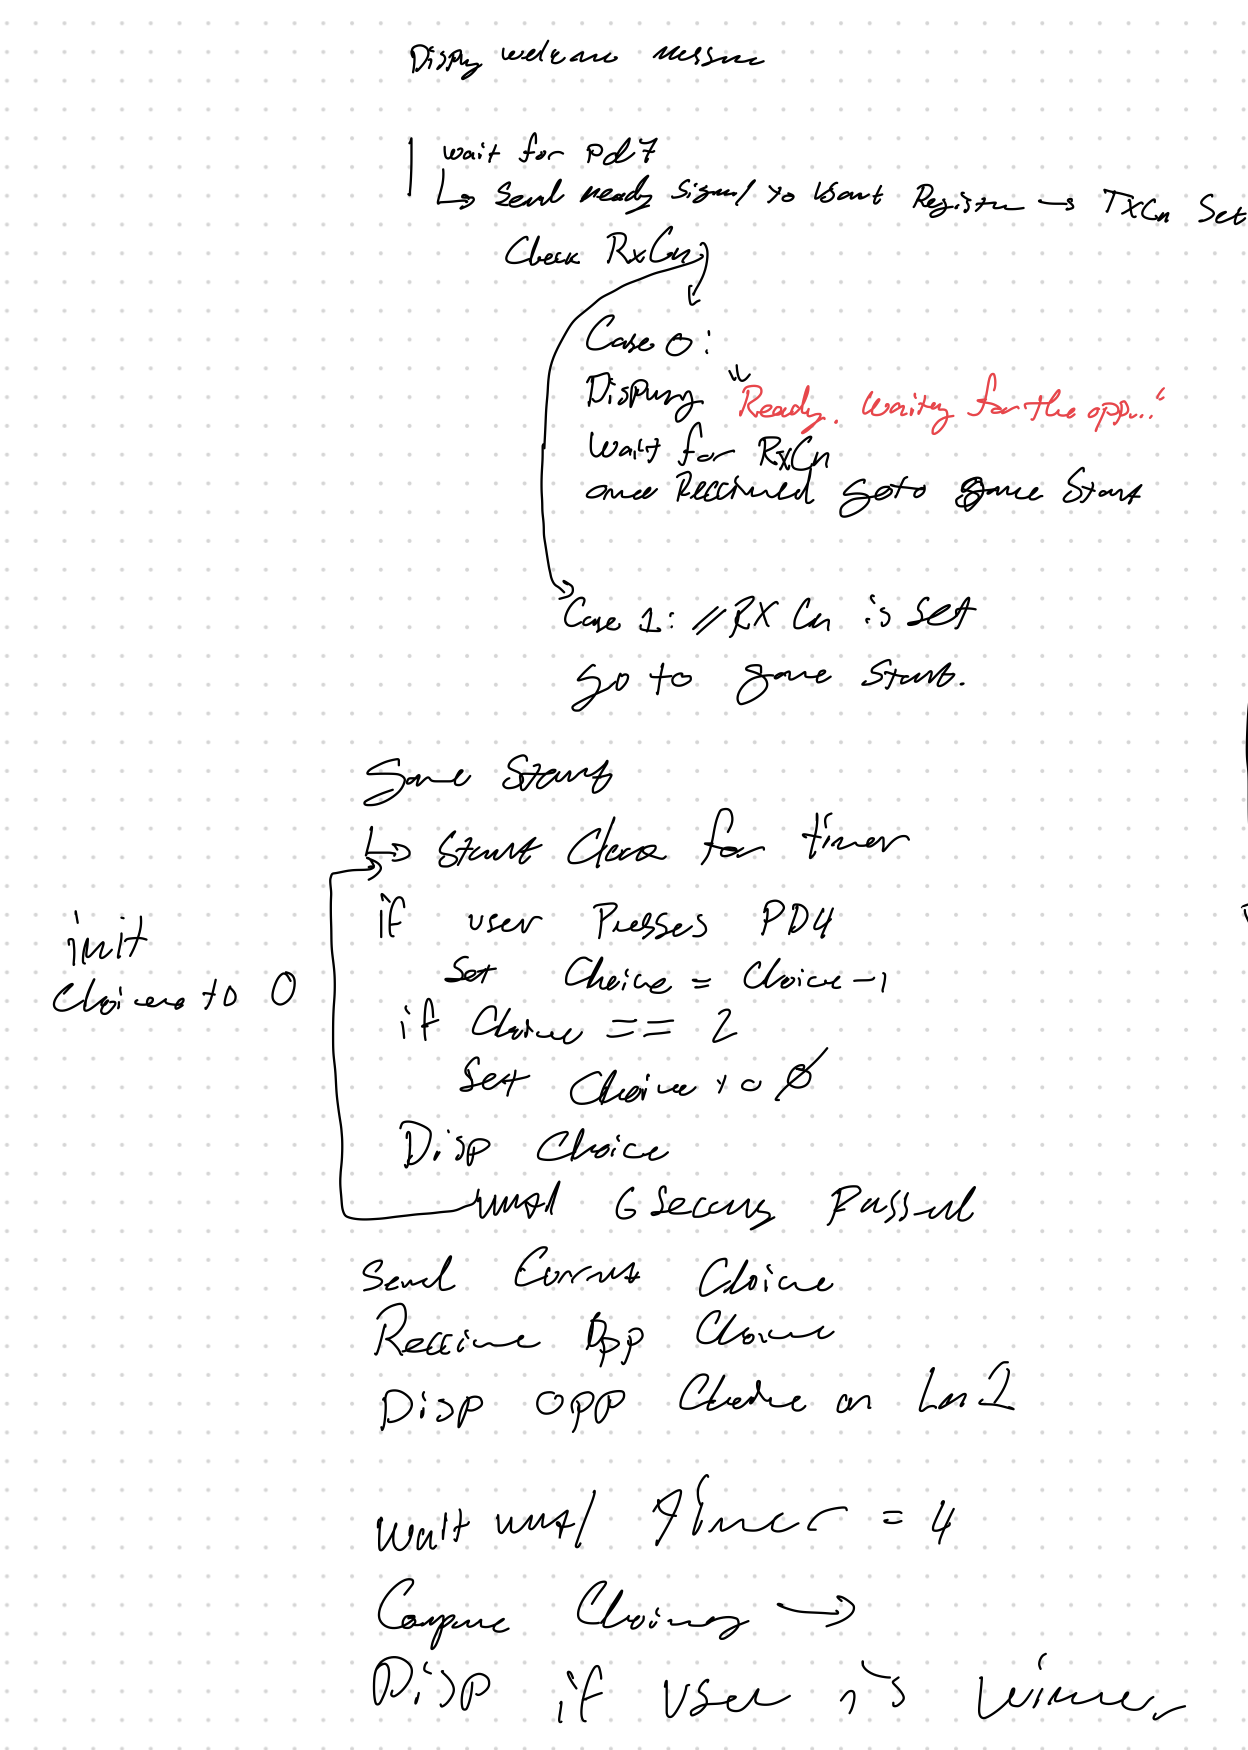
\includegraphics[width=8cm, height=10cm]{flowchart.png}
	\linebreak
\end{figure}

\section{Assembly Overview}
As for the Assembly program an overview can be seen below. 

\subsection{Internal Register Definitions and Constants}
many different internal registers were used for this lab. Those include a multi-purpose register, 2 count registers (inner and outer) for counting lines on the LCD, a zero register to compare to, userChoice to hold the user rock paper scissors choice, tmrcnt a timer count register, button; a register to denounce the button, and oldbut, somewhere to hold the old button signal label. Additionally send ready was initialized to \$FF and the LCD data memory locations were saved to their corresponding names.

\subsection{Interrupt Vectors}
no interrupt vectors were included in this assignment. 
\subsection{Initialization Routine}
The initialization routine was quite complex as it had to setup the USART registers and enable the use of USART. All of the standard initialization parts are there, such as the initialization of the stack pointer, port B for output, Port D for input and the LCD. In addition to setting the baud rate for the USART, an additional timer counter was used to count on the LEDs.

\subsection{Main Routine}
The main program is quite simple as it first writes the welcome text to the LCD, next it querys for button 7. Once button 7 is pressed it makes sure it is connected to another board over USART. Once the key has been sent and received by both parties the mainprogram jumps into the game start routine:


\subsection{Subroutines}
	\subsection{USART\_TX}
	This subroutine is responsible for sending the USART signal cleanly
	\subsection{USART\_RX}
	This subroutine is responsible for receiving a sent USART signal.

	\subsubsection{GAMESTART}
	This subroutine takes care of most of the actual gameplay that occurs while the two boards are communicating. this includes getting the users choice, looping trough timers. Changing the LEDs, and checking to see who won.
	 
	
	\subsubsection{WRITESCREEN}
	The Writescreen subroutine writes the queried data to the LCD. the input for this subroutine is 2 registers, those being ilcnt and olcnt.
	
	\subsubsection{STARTTIMER}
	This function starts the 1.5 second timer and will end and set the timer flag when it finishes. 
	
	\subsection{SMALLWAIT}
	This function waits a small amount of time to allow for debouching of the button input of the methods outlined above.
	

\section{Testing}
Tested Each button press and compared to external calculations.
\begin{table}[h]
	\centering
	\begin{tabular}{|l|l|l|ll}
		\cline{1-3}
		Case & Expected & Actual meet expected &  &  \\ \cline{1-3}
	d4	&rock-> paper-> scissors&	\checkmark  &  \\ \cline{1-3}
	d5	&nothing&	\checkmark	&  \\ \cline{1-3}
	d6	&nothing&	\checkmark  &  \\ \cline{1-3}
	d7	&starts the game&	\checkmark	&  \\ \cline{1-3}
	
%		&          &                      &  &  \\ \cline{1-3}
	\end{tabular}
\caption{Assembly Testing Cases}
\end{table}

\section{Study Questions}
\begin{enumerate}
   \item NONE!
    
       
    
\end{enumerate}

\section{Difficulties}
This lab was quite difficult, mainly due to the fact of how verbose the manual was, and also the fact that the manual has some example code that does not work when applied directly. This caused major problems for us however we eventually found what we needed to do to fix it.

\section{Conclusion}
In conclusion, this lab allowed the student to experiment with sending data over USART and allowed us to play a game using 2 different micro controllers. It was challenging however it also taught many students how not to procrastinate and plan their projects out so they can turn them in on time.

\pagebreak

\section{Source Code}%
\lstinputlisting
[
caption=Assembely Script,
language={[x86masm]Assembler},
numbers =left,
rulesepcolor=\color{blue}
]{../Lab7Assm/Lab7Assm/main.asm}





\end{document}